\section{Traffic Patterns \label{sec:traffic}}

In order to evaluate the performance of interconnection networks, \emph{synthetic
workloads} can be generated. These are a simplification of real execution workloads,
but they capture the important \emph{spatial} and \emph{temporal} elements of
them. With the XK-XMP-64, we are interested in the temporal characteristics of
different traffic patterns and the congestion that they induce over the network.

\subsection{Permutation Patterns}

Synthetic traffic patterns are commonly considered as a permutation $\pi$, which
provides a one-to-one mapping from source addresses $s$ to destination addresses
$d$: $$d = \pi(s).$$ Because permutation traffic concentrates load on individual
source-destination pairs, they provide good stress-testing \cite{dally04}. 

Bit permutations calculate each bit of the destination address $d_i$ as a
function of one bit of the source address $s_i$ such that $$d_i = s_{f(i) \oplus
g(i)}.$$ The following bit permutations were used to evaluate performance.
In all cases, $b$ is the number of bits in the pattern, in the case of
hypercube identifiers $b=d$.

\begin{itemize}

\item {\bf Shuffle.} A Fast Fourier Transform or sorting algorithm will
demonstrate communications characteristic of the shuffle permutation:
$$d_i=s_{i-1\mod b}.$$ 
Equivalently, the identifier is circularly shifted by 1-bit.

\item {\bf Transpose.} Matrix transpose or corner-turn operations induce the
transpose permutation: $$d_i = s_{i+\frac{b}{2}\mod b}.$$ This is equivalent to
a circular shift of an $b$-bit identifier by $b/2$.  The transpose permutation
is a worst case for a hypercube network as it causes all source-destination
pairs to be separated by the full diameter of the network, and hence all nodes
to be maximally loaded.  For the XK-XMP-64 as are interested in the four dimensions
of the hypercube, the transpose relates to a circular shift of two, performed on
the four most significant bits.

\item {\bf Bit-complement.} Each bit is negated: $$d_i = \bar{s_i}.$$

\item {\bf Bit-reverse.} The binary representation is reversed: $$d_i = s_{b-i-1}.$$

\item {\bf Random.} Random permutations were also used to provide an
average-case. These differ slightly to random traffic patterns, where each node
is equally likely to send to each destination, possibly resulting in many
sources sending to a single destination.

\end{itemize}

\subsection{Method}

As we are interested in the spatial locality of the traffic permutations,
measurements can be taken from a single burst of traffic between all
source-destination pairs. If this is performed in unison by all nodes, i.e.\
they begin sending at the same instance, then maximum congestion will occur.

To do this it is necessary to perform a global clock synchronisation, so that
they can synchronise their entry into the permutation and calculate the
latencies of messages sent. Measurements are taken over 10,000 runs of the
permutation to ensure values are representative of the underlying process.

We will look at two important elements of the traffic patterns: distribution of
message latencies and average latencies. To look at the latency distribution,
each node records the latency of each message in a set of frequency bins. To
determine the bin ranges, the traffic pattern is simulated for a number of runs
so that all nodes can share a maximum latency value, from which the bin range is
determined. At the end of the experiment, a master node collates the frequency
distributions from all other nodes. To determine average latency, again each
node records total latency and then calculated average latency on completion,
passing values back to the master node for collation into a global average.

For random permutations, each iteration of the experiment is conducted with a
new permutation so that the measurements are unbiased towards some particular
configuration. This is achieved by each node, each iteration, re-shuffling the
permutation, achieving pseudo-randomness using a cyclic redundancy check (CRC)
instruction. An initial global seed value is distributed to all nodes so they
generate the same sequence of random numbers. According to the permutation,
channel end destinations are manually configured during execution.

With regards to the software implementation, each network node consists of two
threads; one sender and one receiver.  This is necessary for message lengths
greater that the buffering between nodes (16 Bytes). As each dimension of the
hypercube is connected by four links, traffic congestion will be highest when
every link is fully utilised. This can be achieved by running 4 pairs of send
and receive processes on each core.  Alternatively, the number of available
links between each processor can be altered by modifying the XN mapping file.

\subsection{Average Latency}

Figure \ref{fig:avglatency} shows the average latency of messages over all
nodes, for varying message lengths. These results were obtained from all 64
nodes, with each core running a single pair of send and receive threads.
Processors are connected with a single link in each dimension to maximise
congestion. Note that there is very little, or even no penalty for sending short
messages.

\begin{figure}
\centering
%\includegraphics[scale=1]{../images/results/averages/MsgSize-Latency.pdf}
% GNUPLOT: LaTeX picture with Postscript
\begingroup
  \makeatletter
  \providecommand\color[2][]{%
    \GenericError{(gnuplot) \space\space\space\@spaces}{%
      Package color not loaded in conjunction with
      terminal option `colourtext'%
    }{See the gnuplot documentation for explanation.%
    }{Either use 'blacktext' in gnuplot or load the package
      color.sty in LaTeX.}%
    \renewcommand\color[2][]{}%
  }%
  \providecommand\includegraphics[2][]{%
    \GenericError{(gnuplot) \space\space\space\@spaces}{%
      Package graphicx or graphics not loaded%
    }{See the gnuplot documentation for explanation.%
    }{The gnuplot epslatex terminal needs graphicx.sty or graphics.sty.}%
    \renewcommand\includegraphics[2][]{}%
  }%
  \providecommand\rotatebox[2]{#2}%
  \@ifundefined{ifGPcolor}{%
    \newif\ifGPcolor
    \GPcolortrue
  }{}%
  \@ifundefined{ifGPblacktext}{%
    \newif\ifGPblacktext
    \GPblacktexttrue
  }{}%
  % define a \g@addto@macro without @ in the name:
  \let\gplgaddtomacro\g@addto@macro
  % define empty templates for all commands taking text:
  \gdef\gplbacktext{}%
  \gdef\gplfronttext{}%
  \makeatother
  \ifGPblacktext
    % no textcolor at all
    \def\colorrgb#1{}%
    \def\colorgray#1{}%
  \else
    % gray or color?
    \ifGPcolor
      \def\colorrgb#1{\color[rgb]{#1}}%
      \def\colorgray#1{\color[gray]{#1}}%
      \expandafter\def\csname LTw\endcsname{\color{white}}%
      \expandafter\def\csname LTb\endcsname{\color{black}}%
      \expandafter\def\csname LTa\endcsname{\color{black}}%
      \expandafter\def\csname LT0\endcsname{\color[rgb]{1,0,0}}%
      \expandafter\def\csname LT1\endcsname{\color[rgb]{0,1,0}}%
      \expandafter\def\csname LT2\endcsname{\color[rgb]{0,0,1}}%
      \expandafter\def\csname LT3\endcsname{\color[rgb]{1,0,1}}%
      \expandafter\def\csname LT4\endcsname{\color[rgb]{0,1,1}}%
      \expandafter\def\csname LT5\endcsname{\color[rgb]{1,1,0}}%
      \expandafter\def\csname LT6\endcsname{\color[rgb]{0,0,0}}%
      \expandafter\def\csname LT7\endcsname{\color[rgb]{1,0.3,0}}%
      \expandafter\def\csname LT8\endcsname{\color[rgb]{0.5,0.5,0.5}}%
    \else
      % gray
      \def\colorrgb#1{\color{black}}%
      \def\colorgray#1{\color[gray]{#1}}%
      \expandafter\def\csname LTw\endcsname{\color{white}}%
      \expandafter\def\csname LTb\endcsname{\color{black}}%
      \expandafter\def\csname LTa\endcsname{\color{black}}%
      \expandafter\def\csname LT0\endcsname{\color{black}}%
      \expandafter\def\csname LT1\endcsname{\color{black}}%
      \expandafter\def\csname LT2\endcsname{\color{black}}%
      \expandafter\def\csname LT3\endcsname{\color{black}}%
      \expandafter\def\csname LT4\endcsname{\color{black}}%
      \expandafter\def\csname LT5\endcsname{\color{black}}%
      \expandafter\def\csname LT6\endcsname{\color{black}}%
      \expandafter\def\csname LT7\endcsname{\color{black}}%
      \expandafter\def\csname LT8\endcsname{\color{black}}%
    \fi
  \fi
  \setlength{\unitlength}{0.0500bp}%
  \begin{picture}(7936.00,4534.00)%
    \gplgaddtomacro\gplbacktext{%
      \csname LTb\endcsname%
      \put(1254,704){\makebox(0,0)[r]{\strut{} 100}}%
      \put(1254,1595){\makebox(0,0)[r]{\strut{} 1000}}%
      \put(1254,2487){\makebox(0,0)[r]{\strut{} 10000}}%
      \put(1254,3378){\makebox(0,0)[r]{\strut{} 100000}}%
      \put(1254,4269){\makebox(0,0)[r]{\strut{} 1e+06}}%
      \put(1386,484){\makebox(0,0){\strut{} 1}}%
      \put(2941,484){\makebox(0,0){\strut{} 10}}%
      \put(4496,484){\makebox(0,0){\strut{} 100}}%
      \put(6050,484){\makebox(0,0){\strut{} 1000}}%
      \put(7605,484){\makebox(0,0){\strut{} 10000}}%
      \put(352,2486){\rotatebox{-270}{\makebox(0,0){\strut{}Average Latency ($\mu s$)}}}%
      \put(4495,154){\makebox(0,0){\strut{}Message size (KB)}}%
    }%
    \gplgaddtomacro\gplfronttext{%
      \csname LTb\endcsname%
      \put(2706,4096){\makebox(0,0)[r]{\strut{}Shuffle}}%
      \csname LTb\endcsname%
      \put(2706,3876){\makebox(0,0)[r]{\strut{}Transpose}}%
      \csname LTb\endcsname%
      \put(2706,3656){\makebox(0,0)[r]{\strut{}Bit-comp}}%
      \csname LTb\endcsname%
      \put(2706,3436){\makebox(0,0)[r]{\strut{}Bit-rev}}%
      \csname LTb\endcsname%
      \put(2706,3216){\makebox(0,0)[r]{\strut{}Random}}%
    }%
    \gplbacktext
    \put(0,0){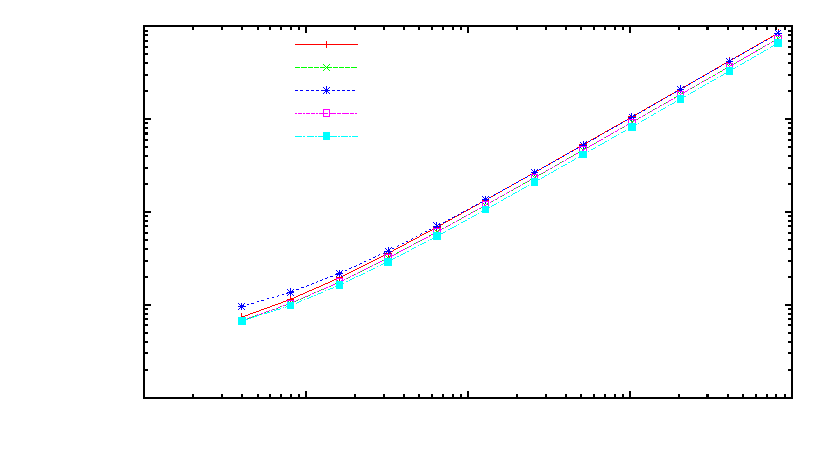
\includegraphics{../images/average-latency.pdf}}%
    \gplfronttext
  \end{picture}%
\endgroup


\caption{Log-log plot of average latency as a function of message size for a 64
nodes.}

\label{fig:avglatency}
\end{figure}

\subsection{Latency Distributions}

Figures \ref{fig:shuffle}, \ref{fig:transpose}, \ref{fig:bitcomp},
\ref{fig:bitrev} and \ref{fig:random} show the latency distributions for a
message length of 32 bytes, with 64 cores and single wire interconnects.

The latency distribution for the random permutation in \fig{random} clearly
shows distributions around each of the 1, 2, 3 and 4 node hops. The
distributions are asymmetric because a hop must always take at least some period
of time, but a message can be delayed in a network for any amount of time.

\begin{figure}
\centering
%\includegraphics[scale=1]{../images/results/histograms/Histogram_SHUFFLE.pdf}
% GNUPLOT: LaTeX picture with Postscript
\begingroup
  \makeatletter
  \providecommand\color[2][]{%
    \GenericError{(gnuplot) \space\space\space\@spaces}{%
      Package color not loaded in conjunction with
      terminal option `colourtext'%
    }{See the gnuplot documentation for explanation.%
    }{Either use 'blacktext' in gnuplot or load the package
      color.sty in LaTeX.}%
    \renewcommand\color[2][]{}%
  }%
  \providecommand\includegraphics[2][]{%
    \GenericError{(gnuplot) \space\space\space\@spaces}{%
      Package graphicx or graphics not loaded%
    }{See the gnuplot documentation for explanation.%
    }{The gnuplot epslatex terminal needs graphicx.sty or graphics.sty.}%
    \renewcommand\includegraphics[2][]{}%
  }%
  \providecommand\rotatebox[2]{#2}%
  \@ifundefined{ifGPcolor}{%
    \newif\ifGPcolor
    \GPcolortrue
  }{}%
  \@ifundefined{ifGPblacktext}{%
    \newif\ifGPblacktext
    \GPblacktexttrue
  }{}%
  % define a \g@addto@macro without @ in the name:
  \let\gplgaddtomacro\g@addto@macro
  % define empty templates for all commands taking text:
  \gdef\gplbacktext{}%
  \gdef\gplfronttext{}%
  \makeatother
  \ifGPblacktext
    % no textcolor at all
    \def\colorrgb#1{}%
    \def\colorgray#1{}%
  \else
    % gray or color?
    \ifGPcolor
      \def\colorrgb#1{\color[rgb]{#1}}%
      \def\colorgray#1{\color[gray]{#1}}%
      \expandafter\def\csname LTw\endcsname{\color{white}}%
      \expandafter\def\csname LTb\endcsname{\color{black}}%
      \expandafter\def\csname LTa\endcsname{\color{black}}%
      \expandafter\def\csname LT0\endcsname{\color[rgb]{1,0,0}}%
      \expandafter\def\csname LT1\endcsname{\color[rgb]{0,1,0}}%
      \expandafter\def\csname LT2\endcsname{\color[rgb]{0,0,1}}%
      \expandafter\def\csname LT3\endcsname{\color[rgb]{1,0,1}}%
      \expandafter\def\csname LT4\endcsname{\color[rgb]{0,1,1}}%
      \expandafter\def\csname LT5\endcsname{\color[rgb]{1,1,0}}%
      \expandafter\def\csname LT6\endcsname{\color[rgb]{0,0,0}}%
      \expandafter\def\csname LT7\endcsname{\color[rgb]{1,0.3,0}}%
      \expandafter\def\csname LT8\endcsname{\color[rgb]{0.5,0.5,0.5}}%
    \else
      % gray
      \def\colorrgb#1{\color{black}}%
      \def\colorgray#1{\color[gray]{#1}}%
      \expandafter\def\csname LTw\endcsname{\color{white}}%
      \expandafter\def\csname LTb\endcsname{\color{black}}%
      \expandafter\def\csname LTa\endcsname{\color{black}}%
      \expandafter\def\csname LT0\endcsname{\color{black}}%
      \expandafter\def\csname LT1\endcsname{\color{black}}%
      \expandafter\def\csname LT2\endcsname{\color{black}}%
      \expandafter\def\csname LT3\endcsname{\color{black}}%
      \expandafter\def\csname LT4\endcsname{\color{black}}%
      \expandafter\def\csname LT5\endcsname{\color{black}}%
      \expandafter\def\csname LT6\endcsname{\color{black}}%
      \expandafter\def\csname LT7\endcsname{\color{black}}%
      \expandafter\def\csname LT8\endcsname{\color{black}}%
    \fi
  \fi
  \setlength{\unitlength}{0.0500bp}%
  \begin{picture}(7936.00,3684.00)%
    \gplgaddtomacro\gplbacktext{%
      \csname LTb\endcsname%
      \put(1342,1012){\makebox(0,0)[r]{\strut{} 0}}%
      \put(1342,1313){\makebox(0,0)[r]{\strut{} 10000}}%
      \put(1342,1614){\makebox(0,0)[r]{\strut{} 20000}}%
      \put(1342,1915){\makebox(0,0)[r]{\strut{} 30000}}%
      \put(1342,2216){\makebox(0,0)[r]{\strut{} 40000}}%
      \put(1342,2516){\makebox(0,0)[r]{\strut{} 50000}}%
      \put(1342,2817){\makebox(0,0)[r]{\strut{} 60000}}%
      \put(1342,3118){\makebox(0,0)[r]{\strut{} 70000}}%
      \put(1342,3419){\makebox(0,0)[r]{\strut{} 80000}}%
      \put(1535,880){\rotatebox{-90}{\makebox(0,0)[l]{\strut{}0}}}%
      \put(2142,880){\rotatebox{-90}{\makebox(0,0)[l]{\strut{}130}}}%
      \put(2749,880){\rotatebox{-90}{\makebox(0,0)[l]{\strut{}260}}}%
      \put(3356,880){\rotatebox{-90}{\makebox(0,0)[l]{\strut{}390}}}%
      \put(3963,880){\rotatebox{-90}{\makebox(0,0)[l]{\strut{}520}}}%
      \put(4570,880){\rotatebox{-90}{\makebox(0,0)[l]{\strut{}650}}}%
      \put(5177,880){\rotatebox{-90}{\makebox(0,0)[l]{\strut{}780}}}%
      \put(5784,880){\rotatebox{-90}{\makebox(0,0)[l]{\strut{}910}}}%
      \put(6391,880){\rotatebox{-90}{\makebox(0,0)[l]{\strut{}1040}}}%
      \put(6998,880){\rotatebox{-90}{\makebox(0,0)[l]{\strut{}1170}}}%
      \put(308,2215){\rotatebox{-270}{\makebox(0,0){\strut{}Count}}}%
      \put(4539,154){\makebox(0,0){\strut{}Message latency (ns)}}%
    }%
    \gplgaddtomacro\gplfronttext{%
    }%
    \gplbacktext
    \put(0,0){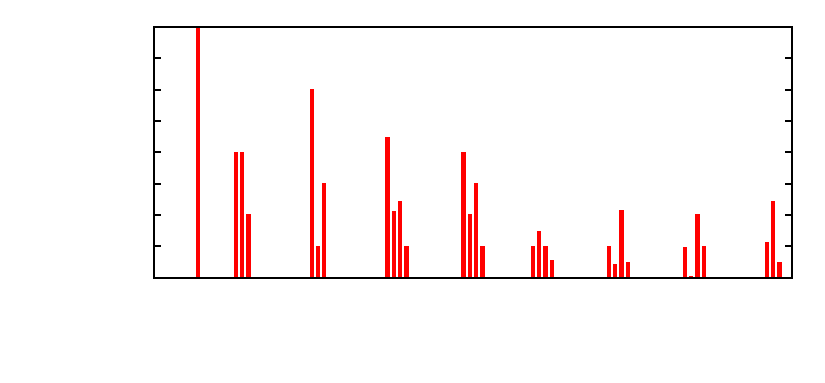
\includegraphics{../images/latency-dist-shuffle.pdf}}%
    \gplfronttext
  \end{picture}%
\endgroup

\caption{Latency distribution for a shuffle permutation}
\label{fig:shuffle}
\end{figure}

\begin{figure}
\centering
%\includegraphics[scale=1]{../images/results/histograms/Histogram_TRANSPOSE.pdf}
% GNUPLOT: LaTeX picture with Postscript
\begingroup
  \makeatletter
  \providecommand\color[2][]{%
    \GenericError{(gnuplot) \space\space\space\@spaces}{%
      Package color not loaded in conjunction with
      terminal option `colourtext'%
    }{See the gnuplot documentation for explanation.%
    }{Either use 'blacktext' in gnuplot or load the package
      color.sty in LaTeX.}%
    \renewcommand\color[2][]{}%
  }%
  \providecommand\includegraphics[2][]{%
    \GenericError{(gnuplot) \space\space\space\@spaces}{%
      Package graphicx or graphics not loaded%
    }{See the gnuplot documentation for explanation.%
    }{The gnuplot epslatex terminal needs graphicx.sty or graphics.sty.}%
    \renewcommand\includegraphics[2][]{}%
  }%
  \providecommand\rotatebox[2]{#2}%
  \@ifundefined{ifGPcolor}{%
    \newif\ifGPcolor
    \GPcolortrue
  }{}%
  \@ifundefined{ifGPblacktext}{%
    \newif\ifGPblacktext
    \GPblacktexttrue
  }{}%
  % define a \g@addto@macro without @ in the name:
  \let\gplgaddtomacro\g@addto@macro
  % define empty templates for all commands taking text:
  \gdef\gplbacktext{}%
  \gdef\gplfronttext{}%
  \makeatother
  \ifGPblacktext
    % no textcolor at all
    \def\colorrgb#1{}%
    \def\colorgray#1{}%
  \else
    % gray or color?
    \ifGPcolor
      \def\colorrgb#1{\color[rgb]{#1}}%
      \def\colorgray#1{\color[gray]{#1}}%
      \expandafter\def\csname LTw\endcsname{\color{white}}%
      \expandafter\def\csname LTb\endcsname{\color{black}}%
      \expandafter\def\csname LTa\endcsname{\color{black}}%
      \expandafter\def\csname LT0\endcsname{\color[rgb]{1,0,0}}%
      \expandafter\def\csname LT1\endcsname{\color[rgb]{0,1,0}}%
      \expandafter\def\csname LT2\endcsname{\color[rgb]{0,0,1}}%
      \expandafter\def\csname LT3\endcsname{\color[rgb]{1,0,1}}%
      \expandafter\def\csname LT4\endcsname{\color[rgb]{0,1,1}}%
      \expandafter\def\csname LT5\endcsname{\color[rgb]{1,1,0}}%
      \expandafter\def\csname LT6\endcsname{\color[rgb]{0,0,0}}%
      \expandafter\def\csname LT7\endcsname{\color[rgb]{1,0.3,0}}%
      \expandafter\def\csname LT8\endcsname{\color[rgb]{0.5,0.5,0.5}}%
    \else
      % gray
      \def\colorrgb#1{\color{black}}%
      \def\colorgray#1{\color[gray]{#1}}%
      \expandafter\def\csname LTw\endcsname{\color{white}}%
      \expandafter\def\csname LTb\endcsname{\color{black}}%
      \expandafter\def\csname LTa\endcsname{\color{black}}%
      \expandafter\def\csname LT0\endcsname{\color{black}}%
      \expandafter\def\csname LT1\endcsname{\color{black}}%
      \expandafter\def\csname LT2\endcsname{\color{black}}%
      \expandafter\def\csname LT3\endcsname{\color{black}}%
      \expandafter\def\csname LT4\endcsname{\color{black}}%
      \expandafter\def\csname LT5\endcsname{\color{black}}%
      \expandafter\def\csname LT6\endcsname{\color{black}}%
      \expandafter\def\csname LT7\endcsname{\color{black}}%
      \expandafter\def\csname LT8\endcsname{\color{black}}%
    \fi
  \fi
  \setlength{\unitlength}{0.0500bp}%
  \begin{picture}(7936.00,3684.00)%
    \gplgaddtomacro\gplbacktext{%
      \csname LTb\endcsname%
      \put(1474,1012){\makebox(0,0)[r]{\strut{} 0}}%
      \put(1474,1313){\makebox(0,0)[r]{\strut{} 20000}}%
      \put(1474,1614){\makebox(0,0)[r]{\strut{} 40000}}%
      \put(1474,1915){\makebox(0,0)[r]{\strut{} 60000}}%
      \put(1474,2216){\makebox(0,0)[r]{\strut{} 80000}}%
      \put(1474,2516){\makebox(0,0)[r]{\strut{} 100000}}%
      \put(1474,2817){\makebox(0,0)[r]{\strut{} 120000}}%
      \put(1474,3118){\makebox(0,0)[r]{\strut{} 140000}}%
      \put(1474,3419){\makebox(0,0)[r]{\strut{} 160000}}%
      \put(1665,880){\rotatebox{-90}{\makebox(0,0)[l]{\strut{}0}}}%
      \put(2259,880){\rotatebox{-90}{\makebox(0,0)[l]{\strut{}130}}}%
      \put(2853,880){\rotatebox{-90}{\makebox(0,0)[l]{\strut{}260}}}%
      \put(3447,880){\rotatebox{-90}{\makebox(0,0)[l]{\strut{}390}}}%
      \put(4041,880){\rotatebox{-90}{\makebox(0,0)[l]{\strut{}520}}}%
      \put(4635,880){\rotatebox{-90}{\makebox(0,0)[l]{\strut{}650}}}%
      \put(5229,880){\rotatebox{-90}{\makebox(0,0)[l]{\strut{}780}}}%
      \put(5823,880){\rotatebox{-90}{\makebox(0,0)[l]{\strut{}910}}}%
      \put(6417,880){\rotatebox{-90}{\makebox(0,0)[l]{\strut{}1040}}}%
      \put(7011,880){\rotatebox{-90}{\makebox(0,0)[l]{\strut{}1170}}}%
      \put(308,2215){\rotatebox{-270}{\makebox(0,0){\strut{}Count}}}%
      \put(4605,154){\makebox(0,0){\strut{}Message latency (ns)}}%
    }%
    \gplgaddtomacro\gplfronttext{%
    }%
    \gplbacktext
    \put(0,0){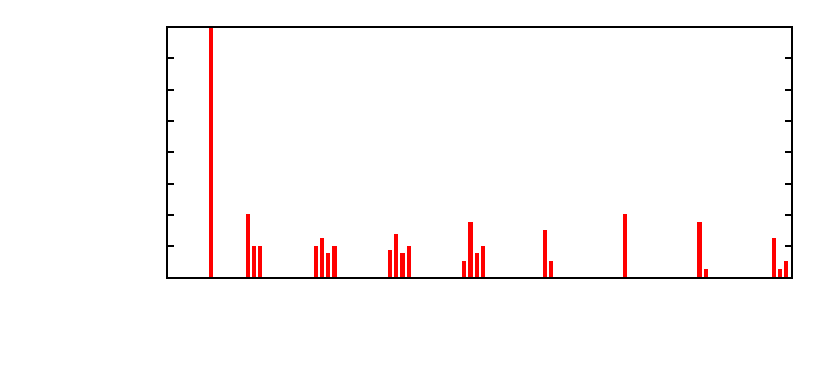
\includegraphics{../images/latency-dist-transpose.pdf}}%
    \gplfronttext
  \end{picture}%
\endgroup

\caption{Latency distribution for a transpose permutation}
\label{fig:transpose}
\end{figure}

\begin{figure}
\centering
%\includegraphics[scale=1]{../images/results/histograms/Histogram_BITCOMP.pdf}
% GNUPLOT: LaTeX picture with Postscript
\begingroup
  \makeatletter
  \providecommand\color[2][]{%
    \GenericError{(gnuplot) \space\space\space\@spaces}{%
      Package color not loaded in conjunction with
      terminal option `colourtext'%
    }{See the gnuplot documentation for explanation.%
    }{Either use 'blacktext' in gnuplot or load the package
      color.sty in LaTeX.}%
    \renewcommand\color[2][]{}%
  }%
  \providecommand\includegraphics[2][]{%
    \GenericError{(gnuplot) \space\space\space\@spaces}{%
      Package graphicx or graphics not loaded%
    }{See the gnuplot documentation for explanation.%
    }{The gnuplot epslatex terminal needs graphicx.sty or graphics.sty.}%
    \renewcommand\includegraphics[2][]{}%
  }%
  \providecommand\rotatebox[2]{#2}%
  \@ifundefined{ifGPcolor}{%
    \newif\ifGPcolor
    \GPcolortrue
  }{}%
  \@ifundefined{ifGPblacktext}{%
    \newif\ifGPblacktext
    \GPblacktexttrue
  }{}%
  % define a \g@addto@macro without @ in the name:
  \let\gplgaddtomacro\g@addto@macro
  % define empty templates for all commands taking text:
  \gdef\gplbacktext{}%
  \gdef\gplfronttext{}%
  \makeatother
  \ifGPblacktext
    % no textcolor at all
    \def\colorrgb#1{}%
    \def\colorgray#1{}%
  \else
    % gray or color?
    \ifGPcolor
      \def\colorrgb#1{\color[rgb]{#1}}%
      \def\colorgray#1{\color[gray]{#1}}%
      \expandafter\def\csname LTw\endcsname{\color{white}}%
      \expandafter\def\csname LTb\endcsname{\color{black}}%
      \expandafter\def\csname LTa\endcsname{\color{black}}%
      \expandafter\def\csname LT0\endcsname{\color[rgb]{1,0,0}}%
      \expandafter\def\csname LT1\endcsname{\color[rgb]{0,1,0}}%
      \expandafter\def\csname LT2\endcsname{\color[rgb]{0,0,1}}%
      \expandafter\def\csname LT3\endcsname{\color[rgb]{1,0,1}}%
      \expandafter\def\csname LT4\endcsname{\color[rgb]{0,1,1}}%
      \expandafter\def\csname LT5\endcsname{\color[rgb]{1,1,0}}%
      \expandafter\def\csname LT6\endcsname{\color[rgb]{0,0,0}}%
      \expandafter\def\csname LT7\endcsname{\color[rgb]{1,0.3,0}}%
      \expandafter\def\csname LT8\endcsname{\color[rgb]{0.5,0.5,0.5}}%
    \else
      % gray
      \def\colorrgb#1{\color{black}}%
      \def\colorgray#1{\color[gray]{#1}}%
      \expandafter\def\csname LTw\endcsname{\color{white}}%
      \expandafter\def\csname LTb\endcsname{\color{black}}%
      \expandafter\def\csname LTa\endcsname{\color{black}}%
      \expandafter\def\csname LT0\endcsname{\color{black}}%
      \expandafter\def\csname LT1\endcsname{\color{black}}%
      \expandafter\def\csname LT2\endcsname{\color{black}}%
      \expandafter\def\csname LT3\endcsname{\color{black}}%
      \expandafter\def\csname LT4\endcsname{\color{black}}%
      \expandafter\def\csname LT5\endcsname{\color{black}}%
      \expandafter\def\csname LT6\endcsname{\color{black}}%
      \expandafter\def\csname LT7\endcsname{\color{black}}%
      \expandafter\def\csname LT8\endcsname{\color{black}}%
    \fi
  \fi
  \setlength{\unitlength}{0.0500bp}%
  \begin{picture}(7936.00,3684.00)%
    \gplgaddtomacro\gplbacktext{%
      \csname LTb\endcsname%
      \put(1342,1012){\makebox(0,0)[r]{\strut{} 0}}%
      \put(1342,1614){\makebox(0,0)[r]{\strut{} 5000}}%
      \put(1342,2216){\makebox(0,0)[r]{\strut{} 10000}}%
      \put(1342,2817){\makebox(0,0)[r]{\strut{} 15000}}%
      \put(1342,3419){\makebox(0,0)[r]{\strut{} 20000}}%
      \put(1535,880){\rotatebox{-90}{\makebox(0,0)[l]{\strut{}0}}}%
      \put(2142,880){\rotatebox{-90}{\makebox(0,0)[l]{\strut{}130}}}%
      \put(2749,880){\rotatebox{-90}{\makebox(0,0)[l]{\strut{}260}}}%
      \put(3356,880){\rotatebox{-90}{\makebox(0,0)[l]{\strut{}390}}}%
      \put(3963,880){\rotatebox{-90}{\makebox(0,0)[l]{\strut{}520}}}%
      \put(4570,880){\rotatebox{-90}{\makebox(0,0)[l]{\strut{}650}}}%
      \put(5177,880){\rotatebox{-90}{\makebox(0,0)[l]{\strut{}780}}}%
      \put(5784,880){\rotatebox{-90}{\makebox(0,0)[l]{\strut{}910}}}%
      \put(6391,880){\rotatebox{-90}{\makebox(0,0)[l]{\strut{}1040}}}%
      \put(6998,880){\rotatebox{-90}{\makebox(0,0)[l]{\strut{}1170}}}%
      \put(308,2215){\rotatebox{-270}{\makebox(0,0){\strut{}Count}}}%
      \put(4539,154){\makebox(0,0){\strut{}Message latency (ns)}}%
    }%
    \gplgaddtomacro\gplfronttext{%
    }%
    \gplbacktext
    \put(0,0){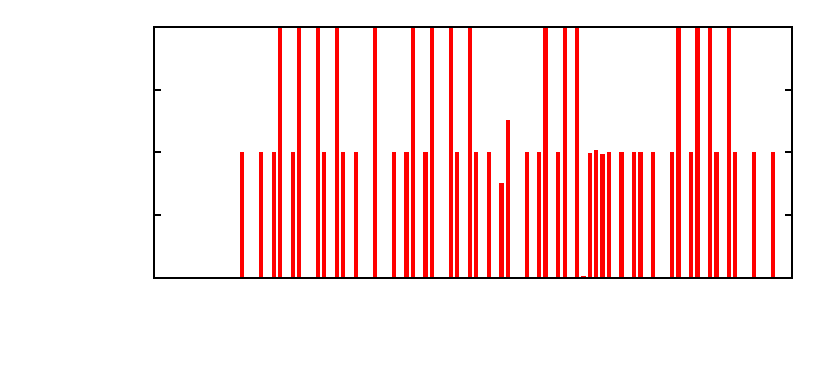
\includegraphics{../images/latency-dist-bitcomp.pdf}}%
    \gplfronttext
  \end{picture}%
\endgroup

\caption{Latency distribution for a bit-complement permutation}
\label{fig:bitcomp}
\end{figure}

\begin{figure}
\centering
%\includegraphics[scale=1]{../images/results/histograms/Histogram_BITREV.pdf}
% GNUPLOT: LaTeX picture with Postscript
\begingroup
  \makeatletter
  \providecommand\color[2][]{%
    \GenericError{(gnuplot) \space\space\space\@spaces}{%
      Package color not loaded in conjunction with
      terminal option `colourtext'%
    }{See the gnuplot documentation for explanation.%
    }{Either use 'blacktext' in gnuplot or load the package
      color.sty in LaTeX.}%
    \renewcommand\color[2][]{}%
  }%
  \providecommand\includegraphics[2][]{%
    \GenericError{(gnuplot) \space\space\space\@spaces}{%
      Package graphicx or graphics not loaded%
    }{See the gnuplot documentation for explanation.%
    }{The gnuplot epslatex terminal needs graphicx.sty or graphics.sty.}%
    \renewcommand\includegraphics[2][]{}%
  }%
  \providecommand\rotatebox[2]{#2}%
  \@ifundefined{ifGPcolor}{%
    \newif\ifGPcolor
    \GPcolortrue
  }{}%
  \@ifundefined{ifGPblacktext}{%
    \newif\ifGPblacktext
    \GPblacktexttrue
  }{}%
  % define a \g@addto@macro without @ in the name:
  \let\gplgaddtomacro\g@addto@macro
  % define empty templates for all commands taking text:
  \gdef\gplbacktext{}%
  \gdef\gplfronttext{}%
  \makeatother
  \ifGPblacktext
    % no textcolor at all
    \def\colorrgb#1{}%
    \def\colorgray#1{}%
  \else
    % gray or color?
    \ifGPcolor
      \def\colorrgb#1{\color[rgb]{#1}}%
      \def\colorgray#1{\color[gray]{#1}}%
      \expandafter\def\csname LTw\endcsname{\color{white}}%
      \expandafter\def\csname LTb\endcsname{\color{black}}%
      \expandafter\def\csname LTa\endcsname{\color{black}}%
      \expandafter\def\csname LT0\endcsname{\color[rgb]{1,0,0}}%
      \expandafter\def\csname LT1\endcsname{\color[rgb]{0,1,0}}%
      \expandafter\def\csname LT2\endcsname{\color[rgb]{0,0,1}}%
      \expandafter\def\csname LT3\endcsname{\color[rgb]{1,0,1}}%
      \expandafter\def\csname LT4\endcsname{\color[rgb]{0,1,1}}%
      \expandafter\def\csname LT5\endcsname{\color[rgb]{1,1,0}}%
      \expandafter\def\csname LT6\endcsname{\color[rgb]{0,0,0}}%
      \expandafter\def\csname LT7\endcsname{\color[rgb]{1,0.3,0}}%
      \expandafter\def\csname LT8\endcsname{\color[rgb]{0.5,0.5,0.5}}%
    \else
      % gray
      \def\colorrgb#1{\color{black}}%
      \def\colorgray#1{\color[gray]{#1}}%
      \expandafter\def\csname LTw\endcsname{\color{white}}%
      \expandafter\def\csname LTb\endcsname{\color{black}}%
      \expandafter\def\csname LTa\endcsname{\color{black}}%
      \expandafter\def\csname LT0\endcsname{\color{black}}%
      \expandafter\def\csname LT1\endcsname{\color{black}}%
      \expandafter\def\csname LT2\endcsname{\color{black}}%
      \expandafter\def\csname LT3\endcsname{\color{black}}%
      \expandafter\def\csname LT4\endcsname{\color{black}}%
      \expandafter\def\csname LT5\endcsname{\color{black}}%
      \expandafter\def\csname LT6\endcsname{\color{black}}%
      \expandafter\def\csname LT7\endcsname{\color{black}}%
      \expandafter\def\csname LT8\endcsname{\color{black}}%
    \fi
  \fi
  \setlength{\unitlength}{0.0500bp}%
  \begin{picture}(7936.00,3684.00)%
    \gplgaddtomacro\gplbacktext{%
      \csname LTb\endcsname%
      \put(1474,1012){\makebox(0,0)[r]{\strut{} 0}}%
      \put(1474,1313){\makebox(0,0)[r]{\strut{} 20000}}%
      \put(1474,1614){\makebox(0,0)[r]{\strut{} 40000}}%
      \put(1474,1915){\makebox(0,0)[r]{\strut{} 60000}}%
      \put(1474,2216){\makebox(0,0)[r]{\strut{} 80000}}%
      \put(1474,2516){\makebox(0,0)[r]{\strut{} 100000}}%
      \put(1474,2817){\makebox(0,0)[r]{\strut{} 120000}}%
      \put(1474,3118){\makebox(0,0)[r]{\strut{} 140000}}%
      \put(1474,3419){\makebox(0,0)[r]{\strut{} 160000}}%
      \put(1665,880){\rotatebox{-90}{\makebox(0,0)[l]{\strut{}0}}}%
      \put(2259,880){\rotatebox{-90}{\makebox(0,0)[l]{\strut{}130}}}%
      \put(2853,880){\rotatebox{-90}{\makebox(0,0)[l]{\strut{}260}}}%
      \put(3447,880){\rotatebox{-90}{\makebox(0,0)[l]{\strut{}390}}}%
      \put(4041,880){\rotatebox{-90}{\makebox(0,0)[l]{\strut{}520}}}%
      \put(4635,880){\rotatebox{-90}{\makebox(0,0)[l]{\strut{}650}}}%
      \put(5229,880){\rotatebox{-90}{\makebox(0,0)[l]{\strut{}780}}}%
      \put(5823,880){\rotatebox{-90}{\makebox(0,0)[l]{\strut{}910}}}%
      \put(6417,880){\rotatebox{-90}{\makebox(0,0)[l]{\strut{}1040}}}%
      \put(7011,880){\rotatebox{-90}{\makebox(0,0)[l]{\strut{}1170}}}%
      \put(308,2215){\rotatebox{-270}{\makebox(0,0){\strut{}Count}}}%
      \put(4605,154){\makebox(0,0){\strut{}Message latency (ns)}}%
    }%
    \gplgaddtomacro\gplfronttext{%
    }%
    \gplbacktext
    \put(0,0){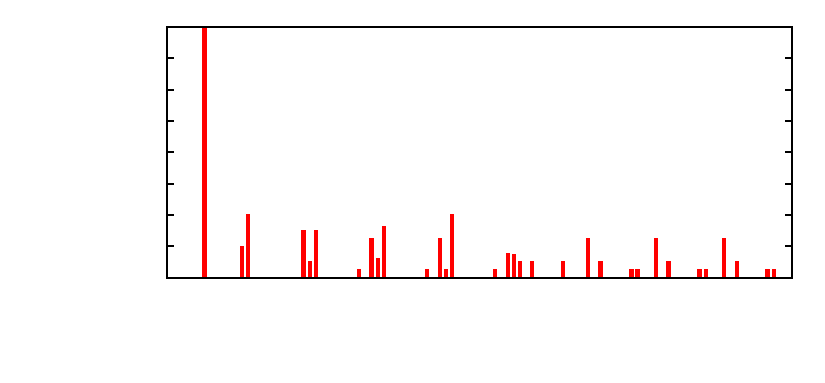
\includegraphics{../images/latency-dist-bitrev.pdf}}%
    \gplfronttext
  \end{picture}%
\endgroup

\caption{Latency distribution for a bit-reverse permutation}
\label{fig:bitrev}
\end{figure}

\begin{figure}
\centering
%\includegraphics[scale=1]{../images/results/histograms/Histogram_RANDOM.pdf}
% GNUPLOT: LaTeX picture with Postscript
\begingroup
  \makeatletter
  \providecommand\color[2][]{%
    \GenericError{(gnuplot) \space\space\space\@spaces}{%
      Package color not loaded in conjunction with
      terminal option `colourtext'%
    }{See the gnuplot documentation for explanation.%
    }{Either use 'blacktext' in gnuplot or load the package
      color.sty in LaTeX.}%
    \renewcommand\color[2][]{}%
  }%
  \providecommand\includegraphics[2][]{%
    \GenericError{(gnuplot) \space\space\space\@spaces}{%
      Package graphicx or graphics not loaded%
    }{See the gnuplot documentation for explanation.%
    }{The gnuplot epslatex terminal needs graphicx.sty or graphics.sty.}%
    \renewcommand\includegraphics[2][]{}%
  }%
  \providecommand\rotatebox[2]{#2}%
  \@ifundefined{ifGPcolor}{%
    \newif\ifGPcolor
    \GPcolortrue
  }{}%
  \@ifundefined{ifGPblacktext}{%
    \newif\ifGPblacktext
    \GPblacktexttrue
  }{}%
  % define a \g@addto@macro without @ in the name:
  \let\gplgaddtomacro\g@addto@macro
  % define empty templates for all commands taking text:
  \gdef\gplbacktext{}%
  \gdef\gplfronttext{}%
  \makeatother
  \ifGPblacktext
    % no textcolor at all
    \def\colorrgb#1{}%
    \def\colorgray#1{}%
  \else
    % gray or color?
    \ifGPcolor
      \def\colorrgb#1{\color[rgb]{#1}}%
      \def\colorgray#1{\color[gray]{#1}}%
      \expandafter\def\csname LTw\endcsname{\color{white}}%
      \expandafter\def\csname LTb\endcsname{\color{black}}%
      \expandafter\def\csname LTa\endcsname{\color{black}}%
      \expandafter\def\csname LT0\endcsname{\color[rgb]{1,0,0}}%
      \expandafter\def\csname LT1\endcsname{\color[rgb]{0,1,0}}%
      \expandafter\def\csname LT2\endcsname{\color[rgb]{0,0,1}}%
      \expandafter\def\csname LT3\endcsname{\color[rgb]{1,0,1}}%
      \expandafter\def\csname LT4\endcsname{\color[rgb]{0,1,1}}%
      \expandafter\def\csname LT5\endcsname{\color[rgb]{1,1,0}}%
      \expandafter\def\csname LT6\endcsname{\color[rgb]{0,0,0}}%
      \expandafter\def\csname LT7\endcsname{\color[rgb]{1,0.3,0}}%
      \expandafter\def\csname LT8\endcsname{\color[rgb]{0.5,0.5,0.5}}%
    \else
      % gray
      \def\colorrgb#1{\color{black}}%
      \def\colorgray#1{\color[gray]{#1}}%
      \expandafter\def\csname LTw\endcsname{\color{white}}%
      \expandafter\def\csname LTb\endcsname{\color{black}}%
      \expandafter\def\csname LTa\endcsname{\color{black}}%
      \expandafter\def\csname LT0\endcsname{\color{black}}%
      \expandafter\def\csname LT1\endcsname{\color{black}}%
      \expandafter\def\csname LT2\endcsname{\color{black}}%
      \expandafter\def\csname LT3\endcsname{\color{black}}%
      \expandafter\def\csname LT4\endcsname{\color{black}}%
      \expandafter\def\csname LT5\endcsname{\color{black}}%
      \expandafter\def\csname LT6\endcsname{\color{black}}%
      \expandafter\def\csname LT7\endcsname{\color{black}}%
      \expandafter\def\csname LT8\endcsname{\color{black}}%
    \fi
  \fi
  \setlength{\unitlength}{0.0500bp}%
  \begin{picture}(7936.00,3684.00)%
    \gplgaddtomacro\gplbacktext{%
      \csname LTb\endcsname%
      \put(1342,1012){\makebox(0,0)[r]{\strut{} 0}}%
      \put(1342,1253){\makebox(0,0)[r]{\strut{} 5000}}%
      \put(1342,1493){\makebox(0,0)[r]{\strut{} 10000}}%
      \put(1342,1734){\makebox(0,0)[r]{\strut{} 15000}}%
      \put(1342,1975){\makebox(0,0)[r]{\strut{} 20000}}%
      \put(1342,2216){\makebox(0,0)[r]{\strut{} 25000}}%
      \put(1342,2456){\makebox(0,0)[r]{\strut{} 30000}}%
      \put(1342,2697){\makebox(0,0)[r]{\strut{} 35000}}%
      \put(1342,2938){\makebox(0,0)[r]{\strut{} 40000}}%
      \put(1342,3178){\makebox(0,0)[r]{\strut{} 45000}}%
      \put(1342,3419){\makebox(0,0)[r]{\strut{} 50000}}%
      \put(1535,880){\rotatebox{-90}{\makebox(0,0)[l]{\strut{}0}}}%
      \put(2142,880){\rotatebox{-90}{\makebox(0,0)[l]{\strut{}130}}}%
      \put(2749,880){\rotatebox{-90}{\makebox(0,0)[l]{\strut{}260}}}%
      \put(3356,880){\rotatebox{-90}{\makebox(0,0)[l]{\strut{}390}}}%
      \put(3963,880){\rotatebox{-90}{\makebox(0,0)[l]{\strut{}520}}}%
      \put(4570,880){\rotatebox{-90}{\makebox(0,0)[l]{\strut{}650}}}%
      \put(5177,880){\rotatebox{-90}{\makebox(0,0)[l]{\strut{}780}}}%
      \put(5784,880){\rotatebox{-90}{\makebox(0,0)[l]{\strut{}910}}}%
      \put(6391,880){\rotatebox{-90}{\makebox(0,0)[l]{\strut{}1040}}}%
      \put(6998,880){\rotatebox{-90}{\makebox(0,0)[l]{\strut{}1170}}}%
      \put(308,2215){\rotatebox{-270}{\makebox(0,0){\strut{}Count}}}%
      \put(4539,154){\makebox(0,0){\strut{}Message latency (ns)}}%
    }%
    \gplgaddtomacro\gplfronttext{%
    }%
    \gplbacktext
    \put(0,0){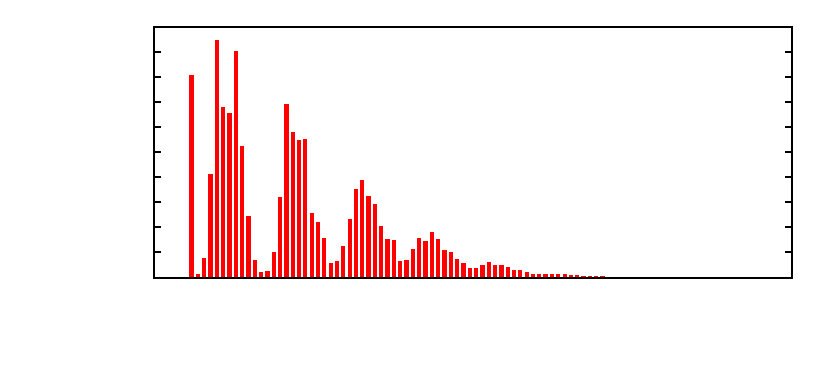
\includegraphics{../images/latency-dist-random.pdf}}%
    \gplfronttext
  \end{picture}%
\endgroup

\caption{Latency distribution for random permutations}
\label{fig:random}
\end{figure}

